
\chapter{Auditory fMRI data}


This data set comprises whole brain BOLD/EPI images acquired on a modified 2T Siemens MAGNETOM Vision system.  Each acquisition consisted of 64  contiguous slices (64x64x64 3mm x 3mm x 3mm voxels). Acquisition took 6.05s, with the scan to scan repeat time (TR) set arbitrarily to 7s.

96 acquisitions were made (TR=7s) from a single subject, in blocks of 6, giving 16 42s blocks. The condition for successive blocks alternated between rest and auditory stimulation, starting with rest. Auditory stimulation was bi-syllabic words presented binaurally at a rate of 60 per minute. The functional data starts at acquisition 4, image \verb!fM00223_004!. Due to T1 effects it is advisable to discard the first few scans (there were no "dummy" lead-in scans). A structural image was also acquired: \verb!sM00223_002!. These images are stored in Analyse format and are available from the SPM site \url{http://www.fil.ion.ucl.ac.uk/spm/data/}. This data set was the first ever collected and analysed in the Functional Imaging Laboratory (FIL) and is known locally as the mother of all experiments (MoAE).

To analyse the data, first create a new directory DIR \newline \verb!eg. c:\home\wpenny\fmri_analysis\auditory!, in which to place the results of your analysis. Then create 3 subdirectories (i) \verb!jobs!, (ii) \verb!classical! and (iii) \verb!bayesian!. As the analysis proceeds these directories will be filled with job-specification files, design matrices and models estimated using classical or Bayesian methods.

Start up matlab, enter your jobs directory and type {\em spm fmri} at the matlab prompt. SPM will then open in fMRI mode with three windows (1) the top-left or `command' window, (2) the bottom-left or `interactive' window and (3) the right-hand or `graphics' window. Analysis then takes place in three major stages (i) spatial pre-processing, (ii) model specification, review and estimation and (iii) inference. These stages organise the buttons in SPM's base window.

\begin{figure}
\begin{center}
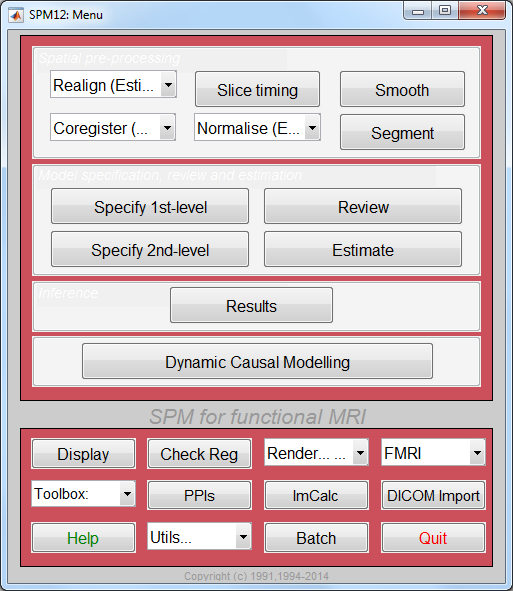
\includegraphics[width=100mm]{auditory/command}
\caption{\em The SPM base window comprises three sections i) spatial pre-processing, (ii) model specification, review and estimation and (iii) inference. \label{command}}
\end{center}
\end{figure}

\section{Spatial pre-processing}

\subsection{Realignment}

Under the spatial pre-processing section of the SPM base window select `Realign' from the `Realign' pulldown menu. This will call up a realignment job specification in the graphics window. Then
\bi
\item{Select `New Realign:Estimate and Reslice'}
\item{Open the newly created `Realign:Estimate and Reslice' option.}
\item{Highlight data, select `New Session', then highlight the newly created `Session' option.} 
\item{Select `Specify Files' and use the SPM file selector to choose all of your functional images eg. `fM000*.img'.}
\item{Save the job file as eg. {\sf DIR/jobs/realign.mat}}.
\item{Press the RUN button in the graphics window.}
\ei

This will run the realign job which will write realigned images into the directory where the functional images are. These new images will be prefixed with the letter `r'. SPM will then plot the estimated time series of translations and rotations shown in Figure~\ref{aud_realign}. These data are also saved to a file eg. \verb!rp_fM00223_004.txt!, so that these variables can be used as regressors when fitting GLMs. This allows movements effects to be discounted when looking for brain activations.

SPM will also create a mean image eg. \verb!meanfM00223_004.img! which will be used in the next step of spatial processing - coregistration.

\begin{figure}
\begin{center}
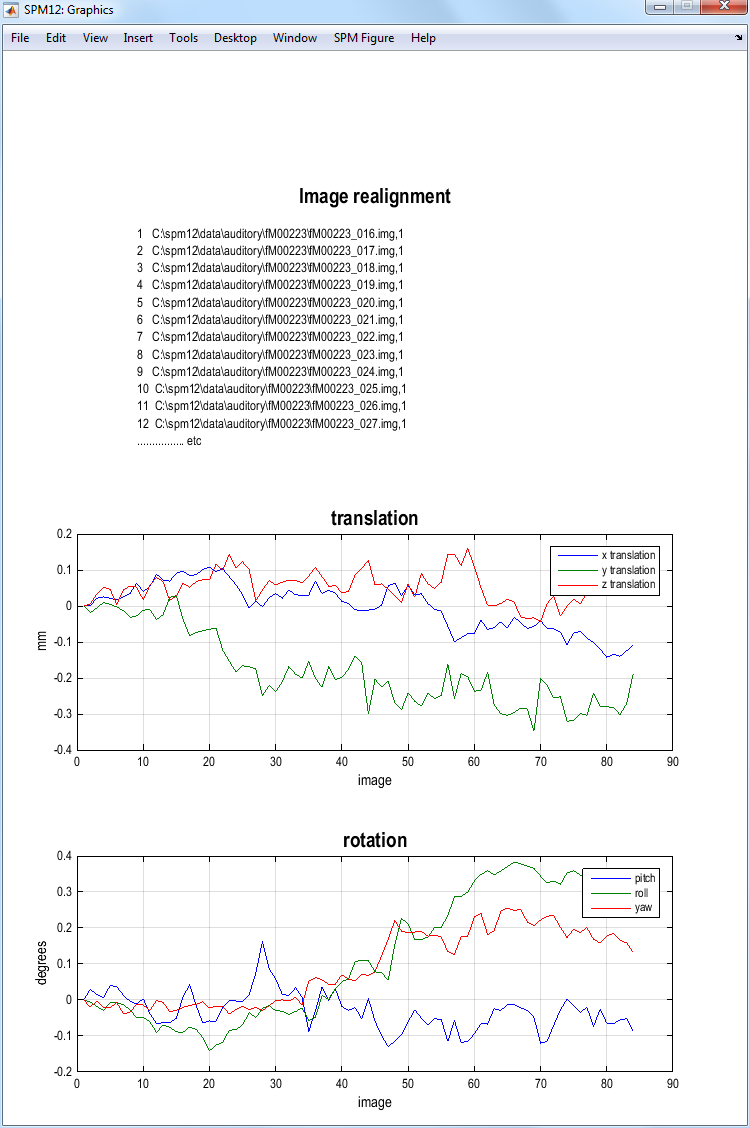
\includegraphics[width=100mm]{auditory/realign}
\caption{\em Realignment of auditory data.\label{aud_realign}}
\end{center}
\end{figure}

\subsection{Coregistration}

Press the `Coreg' button. This will call up the specification of a coregistration job in the graphics window. 

\bi
\item{Select New "Coreg:Estimate"}
\item{Double-click on the newly created Coreg:Estimate}
\item{Highlight `Reference Image' and then select the mean fMRI scan from realignment eg. \verb!meanfM00223_004.img!}
\item{Highlight `Source Image' and then select the structural image eg. \verb!sM00223_002.img!.}
\item{Press the Save button and save the job as {\sf coreg.job}}
\item{Then press RUN}
\ei

SPM will then implement a coregistration between the structural and functional data that maximises the mutual information. The image in figure~\ref{aud_coreg} should then appear in the graphics window. SPM will have changed the header of the source file which in this case is the structural image \verb!sM00223_002.hdr!.
\begin{figure}
\begin{center}
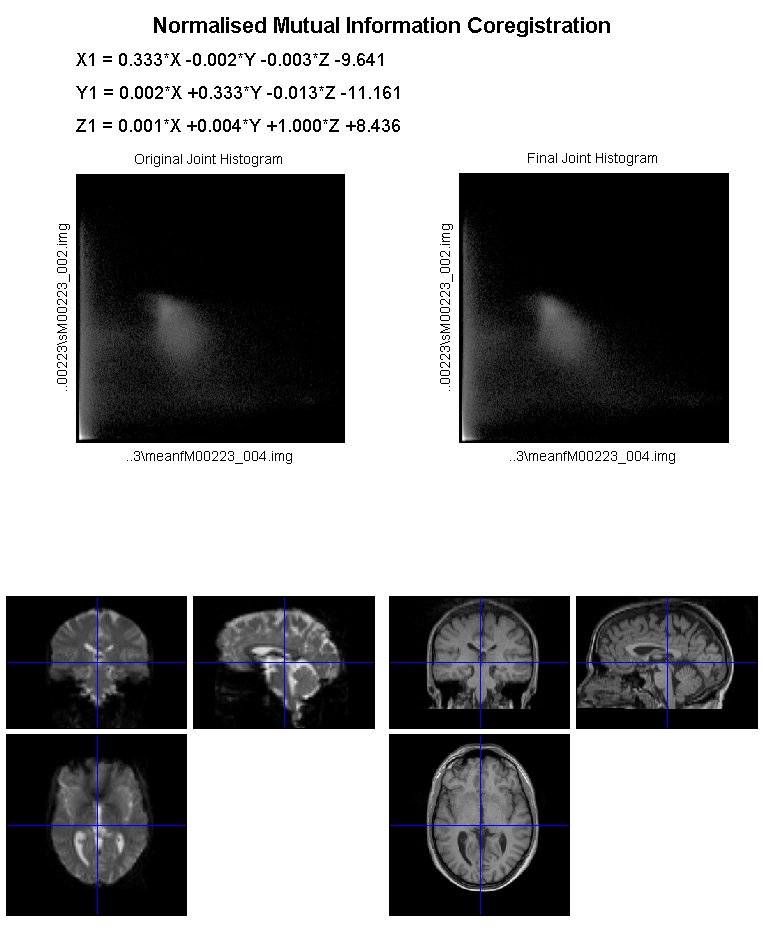
\includegraphics[width=100mm]{auditory/coreg}
\caption{\em Mutual Information Coeregistration  of Auditory data. \label{aud_coreg}}
\end{center}
\end{figure}

The `Check Reg' facility is useful here, to check the results of coregistration. Press the `Check Reg' button in the lower section of the base window and then the select the Reference and Source Images specified above ie \verb!meanfM00223_004.img! and \verb!sM00223_002.img!. SPM will then produce an image like that shown in Figure~\ref{aud_checkreg} in the graphics window. You can then use your mouse to navigate these images to confirm that there is an anatomical correspondence.

\begin{figure}
\begin{center}
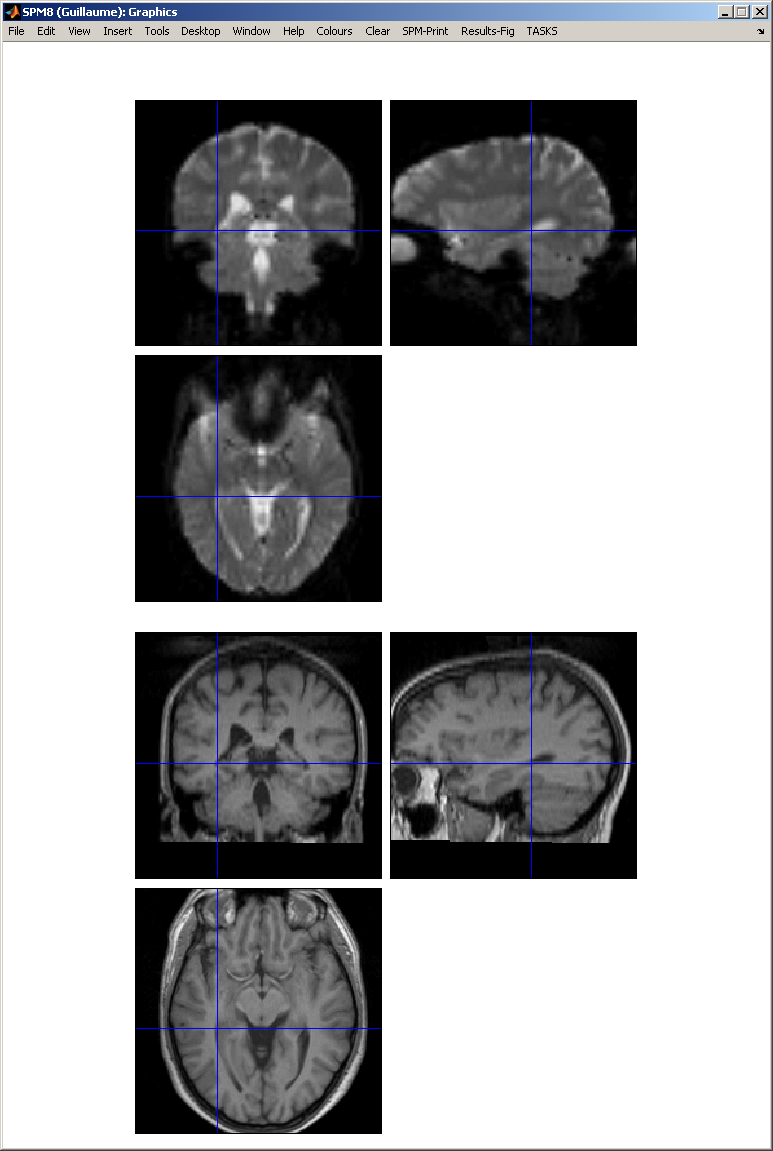
\includegraphics[width=100mm]{auditory/checkreg}
\caption{\em Checking registration of functional and `registered' structural data. \label{aud_checkreg}}
\end{center}
\end{figure}

\subsection{Segmentation}

Press the `Segment' button. This will call up the specification of a segmentation job in the graphics window. Highlight the Data field and then select the subjects registered anatomical image eg. \verb!sM00223_002.img!. Save the job file as {\sf segment.mat} and then press RUN. SPM will segment the structural image using the default tissue probability maps as priors. 

Faster, though perhaps less optimal results can be obtained by eg. reducing the number of Gaussians per class from [2 2 2 4] to eg. [1 1 1 4], increasing the sampling distance from eg. 3 to 4mm. These options can be edited under the `Custom' sub-menu and saved before the job is run. The results obtained in figure \ref{aud_gray} were obtained using the default values.

SPM will create, by default, gray and white matter images and bias-field corrected structural image. These can be viewed using the CheckReg facility as described in the previous section (press segment and select . Figure \ref{aud_gray} shows the gray matter image, \verb!c1sM0023_002.img! along with the original structural.

\begin{figure}
\begin{center}
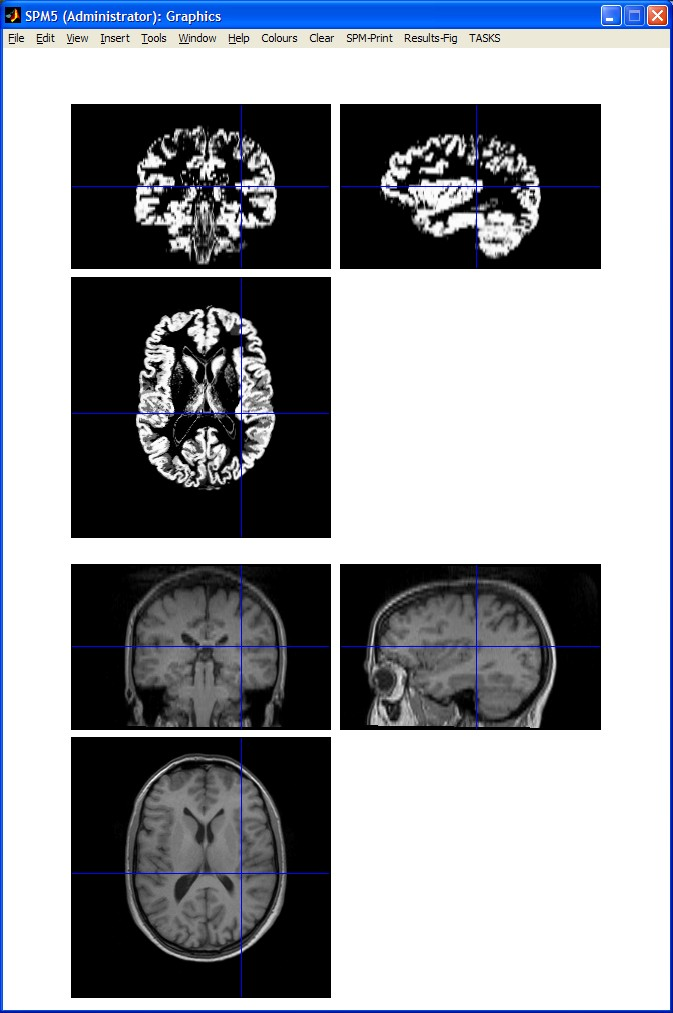
\includegraphics[width=100mm]{auditory/gray}
\caption{\em Gray matter image and `registered' structural image. \label{aud_gray}}
\end{center}
\end{figure}

\begin{figure}
\begin{center}
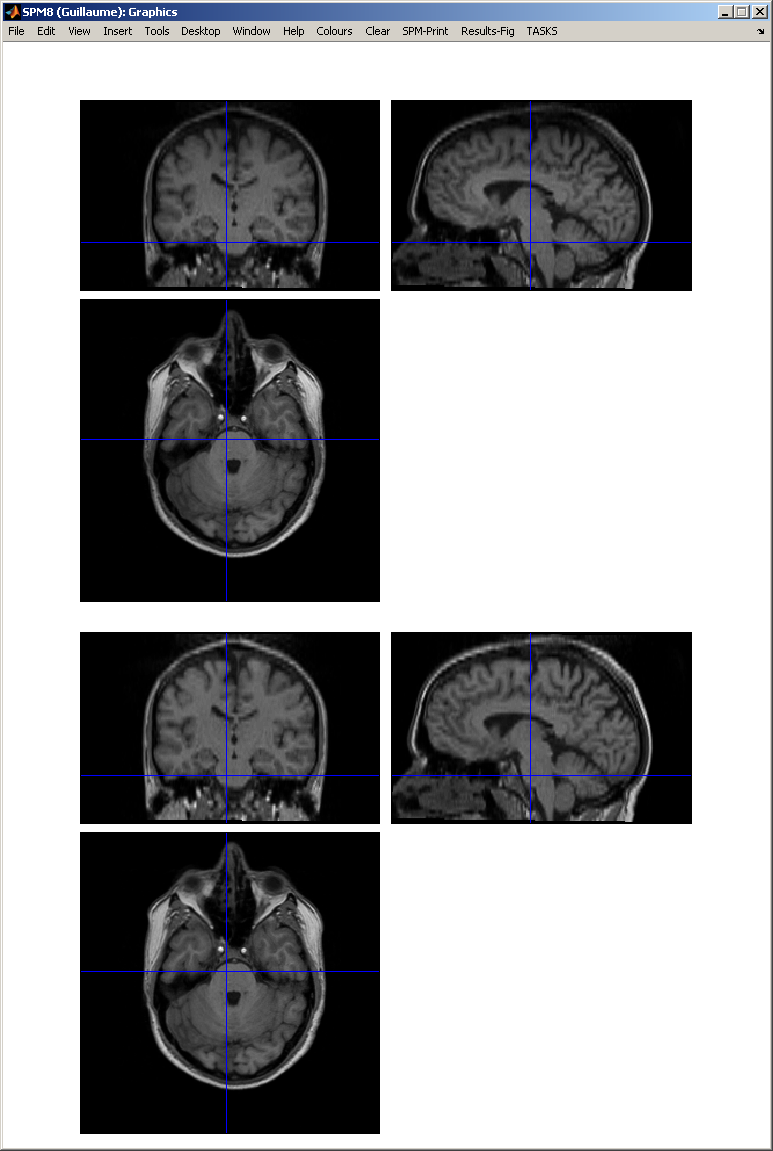
\includegraphics[width=100mm]{auditory/bias}
\caption{\em Structural image (top) and bias-corrected structural image (bottom). Notice that the original structural is darker at the top than at the bottom. This non-uniformity has been removed in the bias-corrected image. \label{aud_bias}}
\end{center}
\end{figure}

SPM will also write a spatial normalisation eg. \verb!sM00223_0020_seg_sn.mat! and inverse spatial normalisation parameters \verb!sM00223_0020_seg_inv_sn.mat! to files in the original structural directory. These can be used to normalise the functional data. 

\subsection{Normalize}

Press the `Normalize' button. This will call up the specification of a normalise job in the graphics window. 

\bi
\item{Select a New "Normalise:Write" field. This allows previously estimated warps to be applied to a series of images.}
\item{Highlight `Data', select New "Subject"}
\item{Open `Subject', highlight `Parameter File' and select the \verb!sM00223_0020_seg_sn.mat! file that you created in the previous section}
\item{Highlight images to write and select all of the realigned functional images `rfM000*.img'. Note: This can be done efficiently by changing the filter in the SPM file selector to \verb!^r.*!. SPM will then only list those files beginning with the letter $r$ ie. those that have been realigned. You can then right click over the listed files, choose `Select all' and press `Done'.}
\item{Open `Writing Options', and change `Voxel sizes' from [2,2,2] to [3,3,3].\footnote{This step is not strictly necessary. It will write images out at a resolution closer to that at which they were acquired. This will speed up subsequent analysis and is necessary, for example, to make Bayesian fMRI analysis computationally efficient.}}
\item{Press `Save', save the job as normalise.mat and then press `Run'.}
\ei

SPM will then write spatially normalised files to the functional data directory. These files have the prefix `w'.

If you wish to superimpose a subject's functional activations on their own anatomy\footnote{Beginners may wish to skip this step, and instead just superimpose functional activations on an `average structural image'.} you will also need to apply the spatial normalisation parameters to their (bias-corrected) anatomical image. To do this

\bi
\item{Press `Normalise', select New "Normalise:Write"}
\item{Open `Normalise: Write', highlight `Data', select New "Subject"}
\item{Open `Subject'}
\item{Highlight `Parameter File', select the  \verb!sM00223_0020_seg_sn.mat! file that you created in the previous section, press `Done'.}
\item{Highlight `Images to Write', select the bias-corrected structural eg. \verb!msM00223_002.img!, press `Done'.}
\item{Open `Writing Options', select voxel sizes and change the default [2 2 2] to [1 1 3] which corresponds to the original resolution of the images.}
\item{Save the job as \verb!norm_struct.mat! and press `Run'}.
\ei

\subsection{Smoothing}

Press the `Smooth' button\footnote{The smoothing step is unnecessary if you are only interested in Bayesian analysis of your functional data.}. This will call up the specification of a smooth job in the graphics window.

\bi
\item{Open `Smooth', select `Images to Smooth' and then select the spatially normalised files created in the last section eg. {\sf wrfM000*.img}. }
\item{Highlight, `FWHM' and change [8 8 8] to [6 6 6]. This will smooth the data by 6mm in each direction.}
\item{Save the job as {\sf smooth.mat} and press `Run'.}
\ei

\begin{figure}
\begin{center}
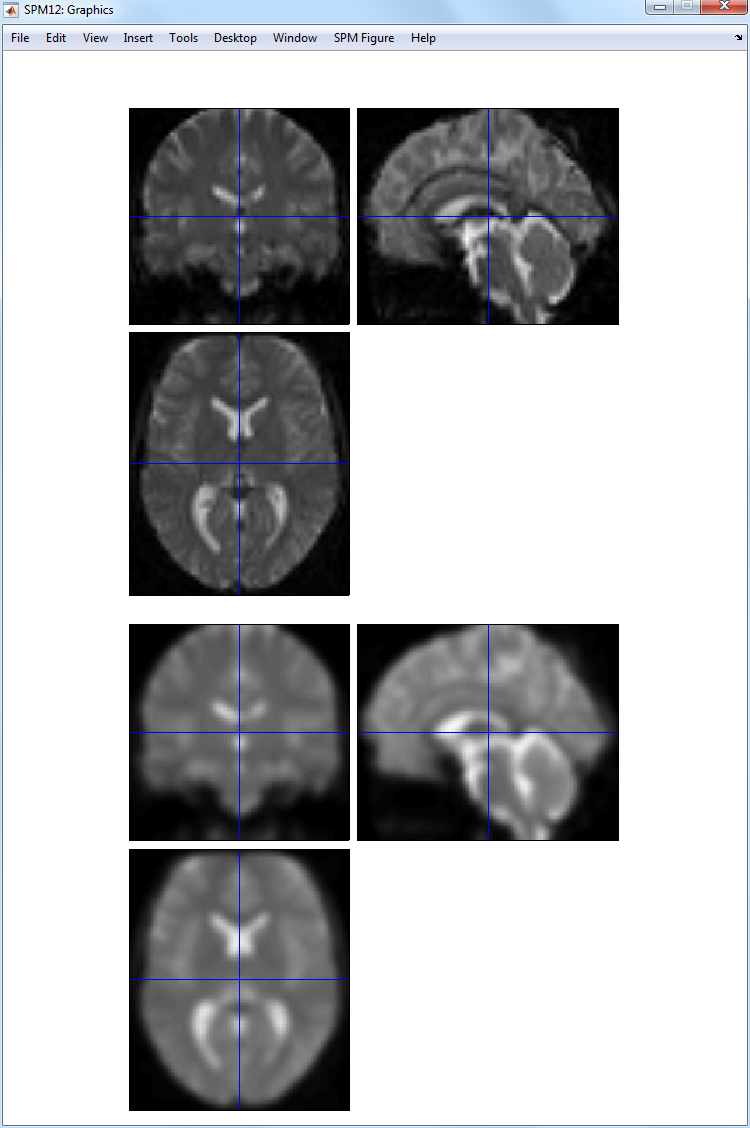
\includegraphics[width=100mm]{auditory/smooth}
\caption{\em Functional image (top) and 6mm-smoothed functional image (bottom). These images were obtained using SPM's `CheckReg' facility. \label{aud_smooth}}
\end{center}
\end{figure}

\section{Model specification, review and estimation}

To avoid T1 effects in the initial scans of an fMRI time series we recommend discarding the first few scans. To make this example simple, we'll discard the first complete cycle (12 scans, 04-15), leaving 84 scans, image files 16-99. This is best done by moving these files to a different directory.

Press the `Specify 1st-level' button. This will call up the specification of an fMRI specification job in the graphics window. Then

\bi
\item{Open the fMRI model specification option}
\item{Open the `Timing parameters' option}
\item{Highlight `Units for design' and select `Scans'}
\item{Highlight `Interscan interval' and enter 7}
\item{Highlight `Data and Design' and select `New Subject/Session'. Then open the newly created `Subject/Session' option.}
\item{Highlight `Scans' and use SPM's file selector to choose the 84 smoothed, normalised functional images ie  \verb!swrfM00223_016.img - *_099.img!. These can be selected easily using the \verb!^s.*'! filter, and select all (provided you have moved the scans 4 to 15 into a different directory). Then press `Done'.}
\item{Highlight `Condition' and select `New condition'}
\item{Open the newly created `Condition' option. Highlight `Name' and enter `active'. Highlight `Onsets' and enter `6:12:84'. Highlight `Durations' and enter `6'.}
\item{Highlight `Directory' and select the \verb!DIR/classical! directory you created earlier.}
\item{Save the job as \verb!specify.mat! and press `RUN'}
\ei

SPM will then write an \verb$SPM.mat$ file to the \verb!DIR/classical! directory. It will also plot the design matrix, as shown in Figure~\ref{auditory/aud_design}. 

\begin{figure}
\begin{center}
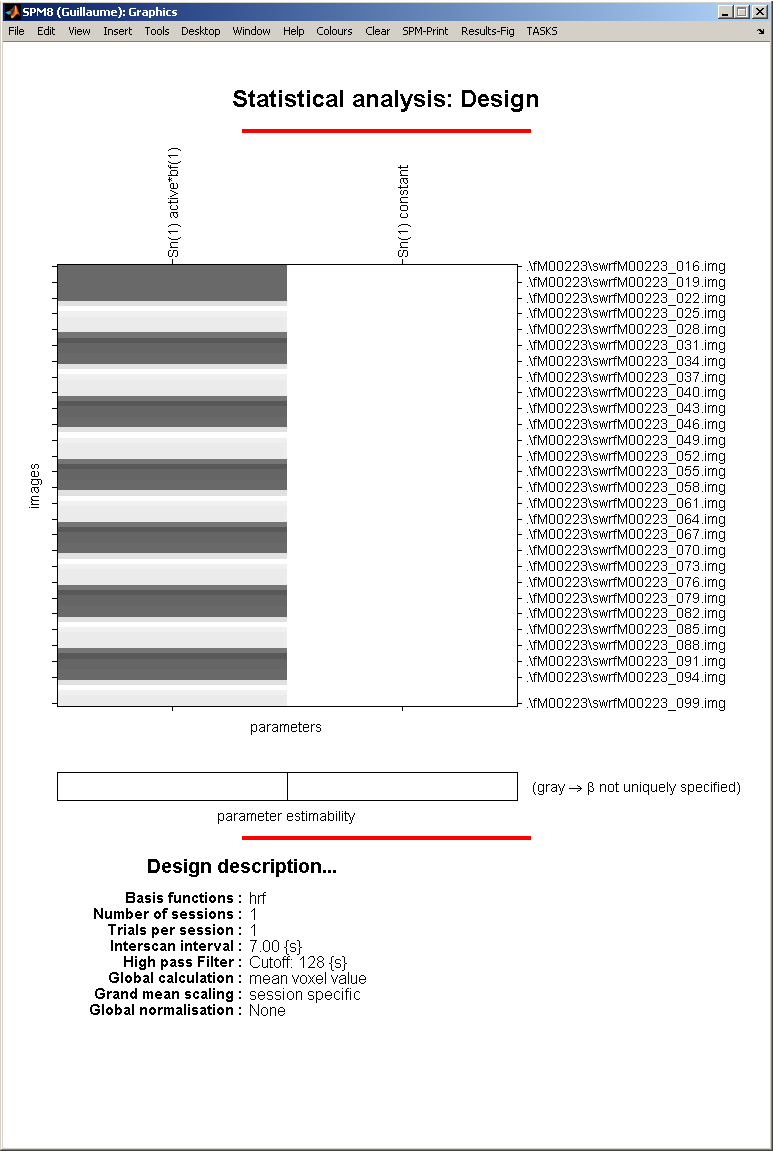
\includegraphics[width=60mm]{auditory/design}
\caption{\em Design matrix. The filenames on the right-hand side of the design matrix indicate the scan associated with each row. \label{aud_design}}
\end{center}
\end{figure}

At this stage it is advisable to check your model specification using SPM's review facility which is accessed via the `Review' button. This brings up a `design' tab on the interactive window clicking on which produces a pulldown menu. If you select the first item `Design Matrix' SPM will produce the image shown in Figure~\ref{aud_design}. If you select `Explore' then `Session 1' then `active', SPM will produce the plots shown in Figure~\ref{aud_explore}.

\begin{figure}
\begin{center}
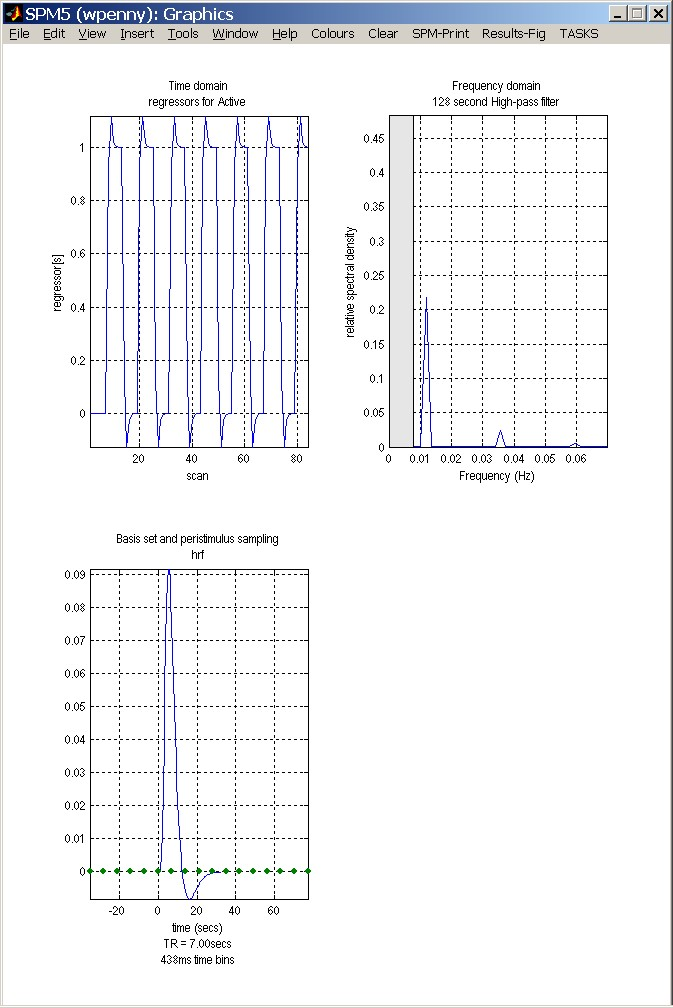
\includegraphics[width=60mm]{auditory/explore}
\caption{\em Exploring the design matrix in Figure~\ref{aud_design}. This shows the time series of the `active' regressor (top left), a frequency domain plot of the active regressor (top right) and the basis function used to convert assumed neuronal activity into hemodynamic activity. In this model we used the default option - the canonical basis function. The frequency domain plot shows that the frequency content of the `active' regressor is above the set frequencies that are removed by the High Pass Filter (HPF) (these are shown in gray - in this model we accepted the default HPF cut-off of 128s or 0.008Hz). \label{aud_explore}}
\end{center}
\end{figure}

If you select the second item on the `Design' tab, `Design Orthogonality', SPM will produce the plot shown in Figure~\ref{aud_orth}. Columns $x_1$ and $x_2$ are orthogonal if the inner product $x_1^T x_2=0$. The inner product can also be written $x_1^T x_2 = |x_1||x_2| cos \theta$ where $|x|$ denotes the length of $x$ and $\theta$ is the angle between the two vectors. So, the vectors will be orthogonal if $cos \theta=0$. The upper-diagonal elements in the matrix at the bottom of figure~\ref{aud_orth} plot $cos\theta$ for each pair of columns in the design matrix. Here we have a single entry.  A degree of non-orthogonality or collinearity is indicated by the gray shading.

\begin{figure}
\begin{center}
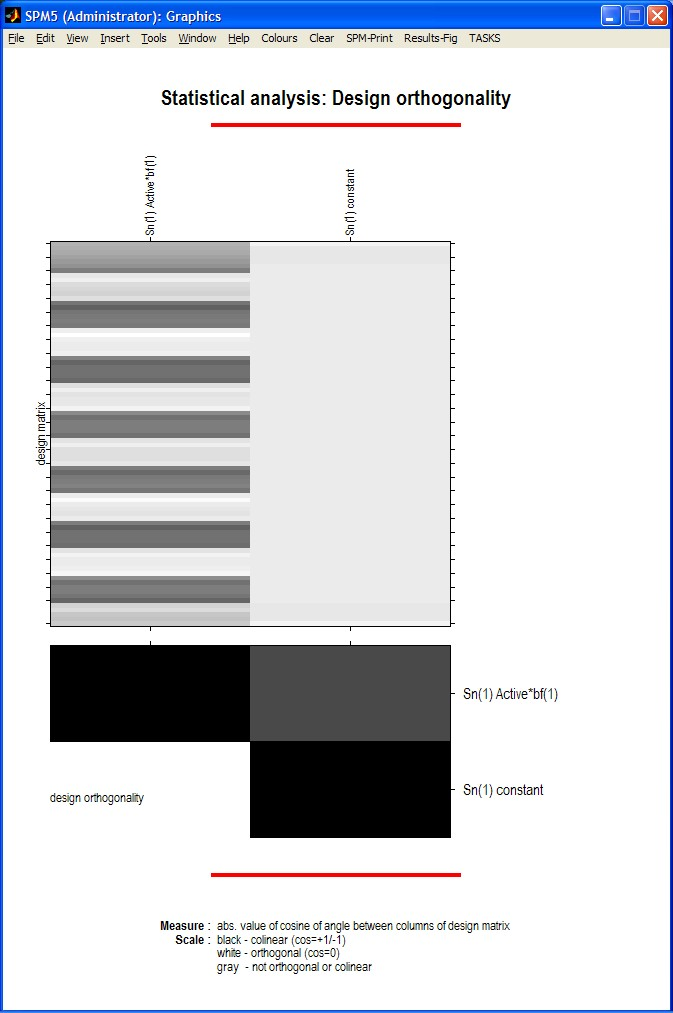
\includegraphics[width=100mm]{auditory/aud_orth}
\caption{\em Design Orthogonality. The description above the first column in the design matrix {\sf Sn(1)Active*bf(1)} means that this column refers to the first session of data (in this analysis there is only 1 session), the name of this condition/trial is `Active' and the trial information has been convolved with the first basis function (the canonical hemodynamic response). The constant regressor for session 1 is referred to as {\sf Sn(1)Constant}. The orthogonality matrix at the bottom indicates a degree of collinearity between regressors. \label{aud_orth}}
\end{center}
\end{figure}

\subsection{Estimate}

Press the `Estimate' button. This will call up the specification of an fMRI estimation job in the graphics window. Then

\bi
\item{Open the `fMRI model estimation' option}
\item{Highlight the `Select SPM.mat' option and then choose the SPM.mat file saved in the classical subdirectory}
\item{Save the job as \verb!estimate.job! and press Run}
\ei

SPM will write a number of files into the selected directory including an \verb!SPM.mat! file.

\section{Inference}

After estimation:

\bi
\item{Press `Results'}
\item{Select the \verb!SPM.mat! file created in the last section}
\ei

\begin{figure}
\begin{center}
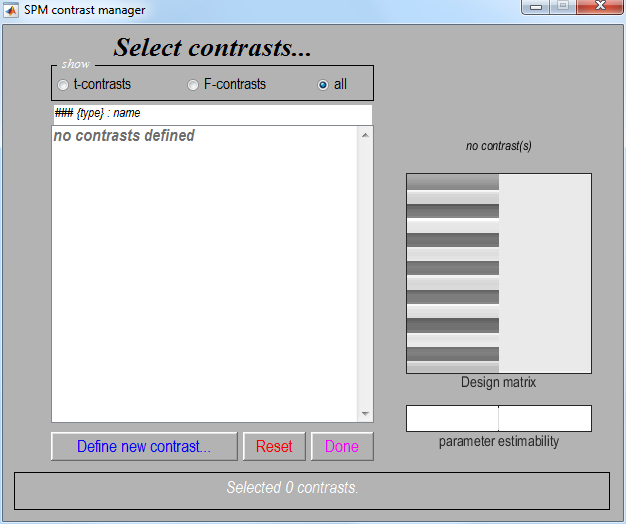
\includegraphics[width=60mm]{auditory/con_man}
\caption{\em The contrast manager}
\end{center}
\end{figure}

This will invoke the contrast manager.

\subsection{Contrast manager}

The contrast manager displays the design matrix (surfable) in the right panel and lists specified contrasts in the left panel. Either 't-contrast' or 'F-contrast' can be selected.  To examine statistical results for condition effects

\bi
\item{Select `Define new contrast'}
\ei
\begin{figure}
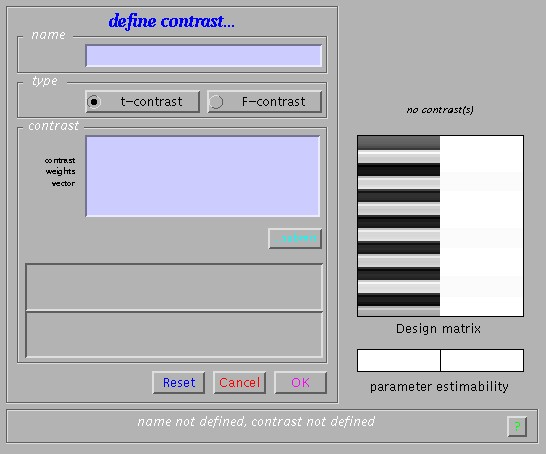
\includegraphics[width=60mm]{auditory/con_man2}
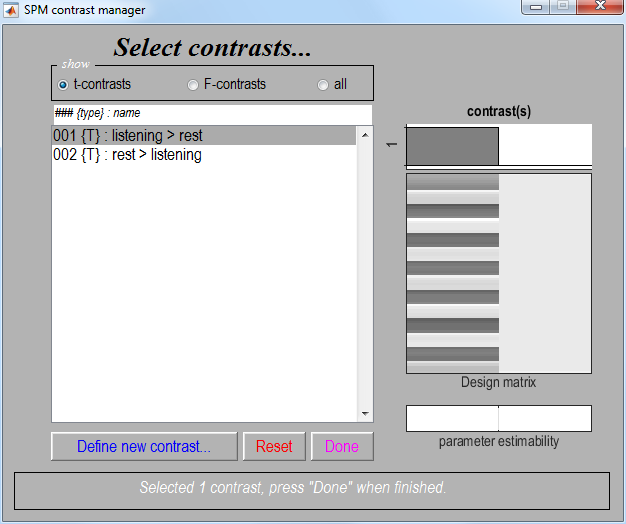
\includegraphics[width=60mm]{auditory/con_man3}
\caption{\em Left: A contrast is entered by specifying the numeric values in the lower window and the name in the upper window. Right: After contrasts have been specified they can be selected.}
\end{figure}

One sided main effects for the active condition (i.e., a one-sided t-test) can be specified (in this example) as '1' (active $>$ rest) and '-1' (rest $>$ active). SPM will accept correct contrasts only. Accepted contrasts are displayed at the bottom of the contrast manager window in green, incorrect ones are displayed in red. To view a contrast

\bi
\item{Select the contrast name e.g., `active $>$ rest'}
\item{Press `Done'}
\ei

\subsection{Masking}

You will then be prompted with

\bi
\item{\em Mask with other contrast ? [Yes/No]}
\item{Specify No.}
\ei

Masking implies selecting voxels specified by other contrasts. If 'yes', SPM will prompt for (one or more) masking contrasts, the significance level of the mask (default p = 0.05 uncorrected), and will ask whether an inclusive or exclusive mask should be used. Exclusive will remove all voxels which reach the default level of significance in the masking contrast, inclusive will remove all voxels which do not reach the default level of significance in the masking contrast. Masking does not affect p-values of the 'target' contrast, it only includes or excludes voxels.

\subsection{Thresholds}

You will then be prompted with

\bi
\item{\em Title for comparison ?}
\item{ Enter eg. 'active  $>$ rest'}
\item{\em Corrected height threshold ? [Yes/No]}
\item{Enter Yes.}
\item{\em p value adjustment to control: [FWE/FDR/none]}
\item{Select FWE}
\item{\em p value(family-wise error)}
\item{Accept the default value, 0.05}
\ei

A Family Wise Error (FWE) is a false positive anywhere in the SPM. Now, imagine repeating your experiment many times and producing SPMs. The proportion of SPMs containing FWEs is the FWE rate. A value of 0.05 implies that 1 in 20 SPMs contains a false positive somewhere in the image. 

If you choose the `none' option above this corresponds to making statistical inferences at the `voxel level'. These use `uncorrected' p values, whereas FWE thresholds are said to use `corrected' p values. SPM's default uncorrected p value is p=0.001. This means that the probability of a false positive at each voxel is 0.001. So if, you have 50,000 voxels you can expect $50,000 \times 0.001 = 50$ false positives in each SPM.

The final option here is False Discovery Rate (FDR). If you set this at 0.1, this means that of all the discoveries you make (ie. above threshold voxels that appear in the SPM) 10\% of them are likely to be false. 

You will then be prompted with

\bi
\item{\em Extent Threshold \{voxels\} [0]}
\item{Accept the default value, 0}
\ei

Entering a value $v$ here will produce SPMs with clusters containing at least $v$ voxels. SPM will then produce the SPM shown in Figure~\ref{aud_spm1}.

\bi
\item{Select `Define new contrast'}
\ei
\begin{figure}
\begin{center}
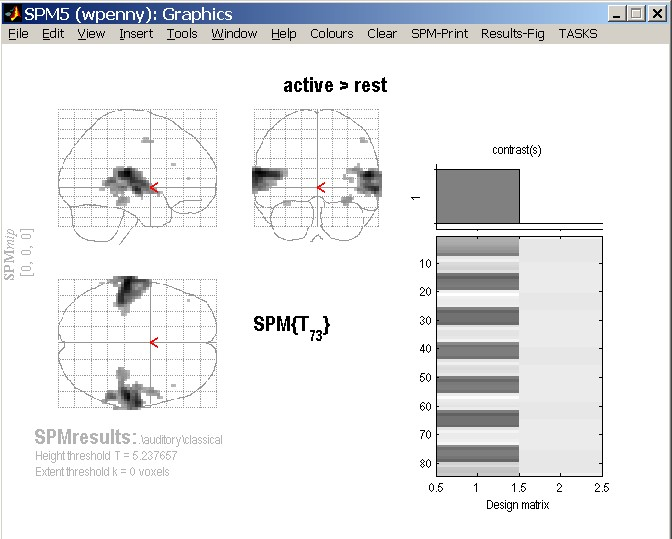
\includegraphics[width=100mm]{auditory/spm1}
\caption{\em SPM showing bilateral activation of auditory cortex. \label{aud_spm1}}
\end{center}
\end{figure}

\subsection{Files}

A number of files are written to the working directory at this time.
Images containing weighted parameter estimates are saved as {\sf con-0002.hdr/img}, {\sf con-0003.hdr/img}, �etc. in the working directory. Images of T-statistics are saved as {\sf spmT-0002.hdr/img}, {\sf spmT-0003.hdr/img} etc., also in the working directory.

\subsection{Maximum Intensity Projections}

SPM displays a Maximum Intensity Projection (MIP) of the statistical map in the graphics window. The MIP is projected on a glass brain in three orthogonal planes. The MIP is surfable: R-clicking in the MIP will activate a pulldown menu, L-clicking  on the red cursor will allow it to be dragged to a new position.

\begin{figure}
\begin{center}
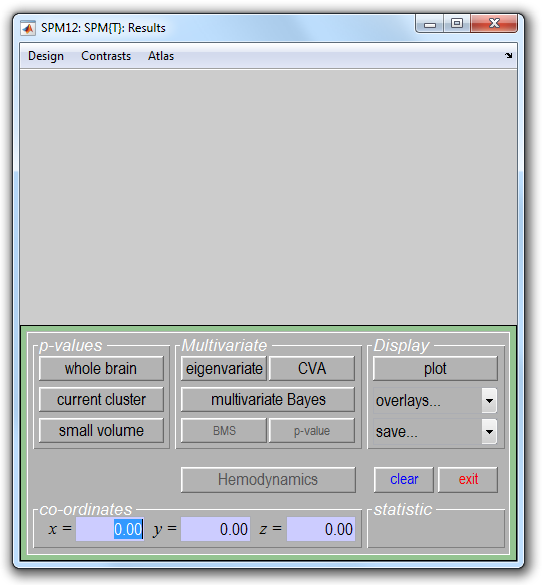
\includegraphics[width=100mm]{auditory/interactive}
\caption{\em SPM's interactive window during results assessment. The `p-values' section is used to produce tables of statistical information. The visualisation section is used to plot responses at a voxel or to visual activations overlaid on anatomical images. The `Regional' section, ie. the VOI button, is used to extract data for subsequent analyses such as assessment of PsychoPhysiological Interactions (PPIs) or Dynamic  Causal Models (DCMs).}
\end{center}
\end{figure}

\subsection{Design matrix}

SPM also displays the design matrix with the selected contrast. The design matrix is also surfable: R-clicking will show parameter names, L-clicking will show design matrix values for each scan. 

In the SPM Interactive window (lower left panel) a button box appears with various options for displaying statistical results (p-values panel) and creating plots/overlays (visualisation panel). Clicking 'Design' (upper left) will activate a pulldown menu as in the 'Explore design' option.

\subsection{Statistical tables}

To get a summary of local maxima, press the `volume' button in the p-values section of the interactive window. This will list all clusters above the chosen level of significance as well as separate ($>$8mm apart) maxima within a cluster, with details of significance thresholds and search volume underneath, as shown in Figure~\ref{aud_volume}

\begin{figure}
\begin{center}
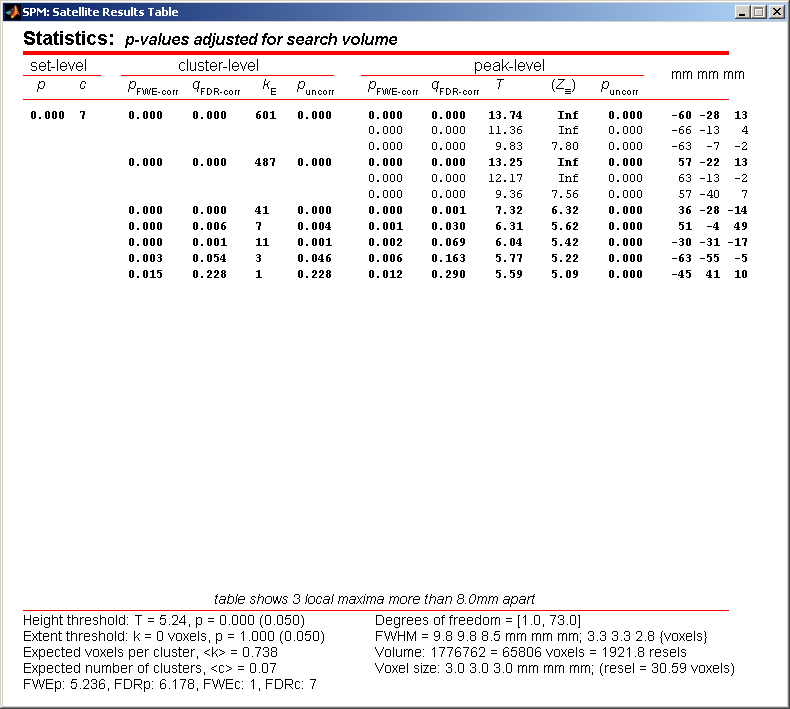
\includegraphics[width=100mm]{auditory/volume}
\caption{\em Volume table for `active $>$ rest' effect. This table of values was created by pressing the `Results-Fig' tab at the top of the graphics window and then pressing the `Volume' button. This displays the table of results in a separate window. \label{aud_volume} }
\end{center}
\end{figure}

The columns in volume table show, from right to left:

\bi
\item{x, y, z (mm): coordinates in Talairach space for each maximum}
\item{voxel-level: the chance (p) of finding (under the null hypothesis) a voxel with this or a greater height (T- or Z-statistic), corrected (FWE or FDR)/ uncorrected for search volume.}
\item{cluster-level: the chance (p) of finding a cluster with this many(ke) or a greater number of voxels, corrected / uncorrected for search volume}
\item{set-level: the chance (p) of finding this (c) or a greater number of clusters in the search volume}
\ei

It is also worth noting that

\bi
\item{The table is surfable: clicking a row of cluster coordinates will move the pointer in the MIP to that cluster, clicking other numbers will display the exact value in the Matlab window (e.g. 0.000 = 6.1971e-07).}
\item{To inspect a specific cluster (e.g., in this example data set, the R auditory cortex), either move the cursor in the MIP (by L-clicking and dragging the cursor, or R-clicking the MIP background which will activate a pulldown menu).}
\item{Alternatively, click the cluster coordinates in the volume table, or type the coordinates in the co-ordinates section of the interactive window.}
\ei

It is also possible to produce tables of statistical information for a single cluster of interest rather than for the whole volume. Firstly, elect the relevant cluster in the MIP and then press the `cluster' button in the p-values section of the interactive window. This will show coordinates and voxel-level statistics for local maxima ($>$4mm apart) in the selected cluster. This table is also surfable.

\subsection{Plotting responses at a voxel}

A voxel can be chosen with co-ordinates corresponding to those in the interactive window. The responses at this voxel can then be plotted using the `Plot' button in the visualisation section of the interactive window. This will provide you with five further options:

\begin{enumerate}
\item{Contrast estimates and 90\% CI: SPM will prompt for a specific contrast (e.g., active$>$rest). The plot will show effect size and 90\% confidence intervals. See eg. Figure~\ref{aud_contrast}}
\item{Fitted responses: Plots adjusted data and fitted response across session/subject. SPM will prompt for a specific contrast and provides the option to choose different ordinates ('an explanatory variable', 'scan or time', or 'user specified'). If 'scan or time', the plot will show adjusted or fitted data with errors added as shown in Figure~\ref{aud_fitted}}
\item{Event-related responses: Plots adjusted data and fitted response across peri-stimulus time.}
\item{Parametric responses}
\item{Volterra kernels}
\end{enumerate}

\begin{figure}
\begin{center}
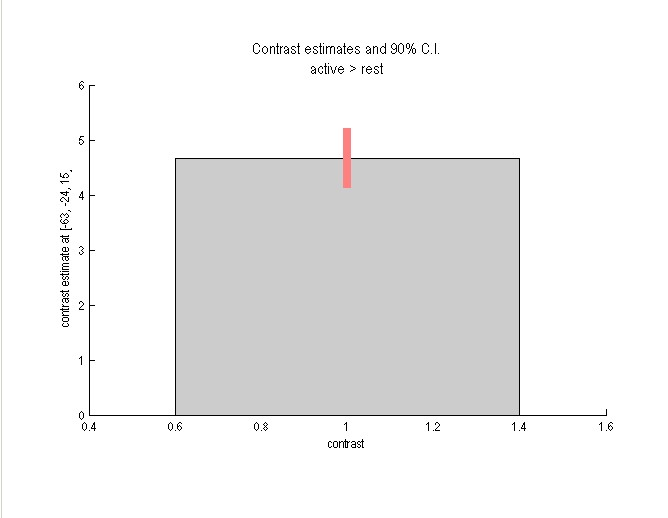
\includegraphics[width=60mm]{auditory/contrast}
\caption{\em Estimated effect size. \label{aud_contrast} }
\end{center}
\end{figure}

\begin{figure}
\begin{center}
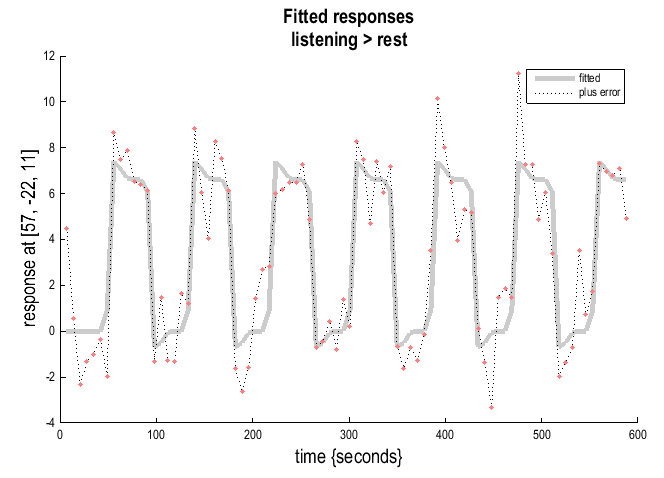
\includegraphics[width=60mm]{auditory/fitted}
\caption{\em Fitted responses. \label{aud_fitted} }
\end{center}
\end{figure}

For plotting event-related responses SPM provides three options

\begin{enumerate}
\item{Fitted response and PSTH (peri-stimulus time histogram): plots mean regressor(s) (ie. averaged over session) and mean signal +/- SE for each peri-stimulus time bin.}
\item{Fitted response and 90\% CI: plots mean regressor(s) along with a 90\% confidence interval.}
\item{Fitted response and adjusted data: plots regressor(s) and individual data (note that in this example the data are shown in columns due to the fixed TR/ISI relationship).}
\end{enumerate}

Its worth noting that

\bi
\item{The values for the fitted response across session/subject for the selected plot can be displayed and accessed in the Matlab window by typing 'Y'. Typing 'y' will display the adjusted data.}
\item{'Adjusted' data = adjusted for confounds (e.g., global flow) and high- and low pass filtering.}
\ei

\subsection{Overlays}

The visualisation section of the interactive window also provides an overlay facility for anatomical visualisation of clusters of activation. Pressing `Overlays' will activate a pulldown menu with three options

\begin{enumerate}
\item{Slices: overlay on three adjacent (2mm) transaxial slices. SPM will prompt for an image for rendering. This could be a canonical image (see {\sf spm-template.man}) or an individual T1/mean EPI image for single-subject analyses.}
\item{Sections: overlay on three intersecting (sagittal, coronal, transaxial) slices. These renderings are surfable: clicking the images will move the crosshair.}
\item{Render: overlay on a volume rendered brain, with options for using a smoothed brain, and old (left) and new (right) style rendering.}
\end{enumerate}

Renderings can be saved as {\sf filename.img} and {\sf filename.hdr} in the working directory by using the {\em write filtered} option. In Figures~\ref{aud_slices}, \ref{aud_sections} and \ref{aud_render} the `active $>$ rest' activation has been superimposed on the spatially normalised, bias-corrected anatomical image \verb!wmsM00223_002.img! created earlier. 

\begin{figure}
\begin{center}
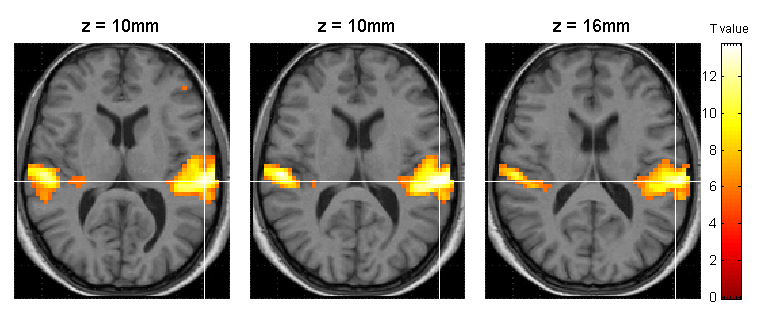
\includegraphics[width=100mm]{auditory/slices}
\caption{\em Slices. \label{aud_slices} }
\end{center}
\end{figure}

\begin{figure}
\begin{center}
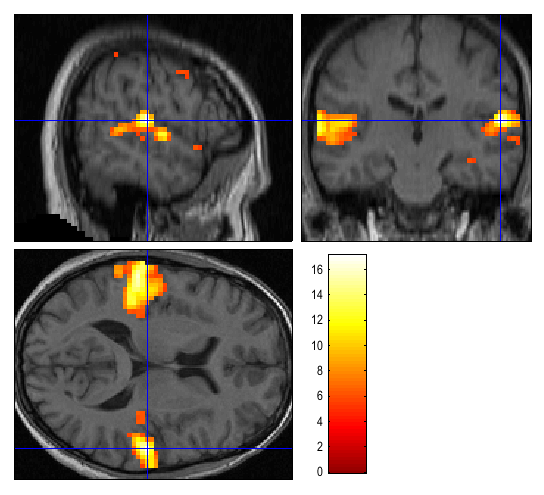
\includegraphics[width=100mm]{auditory/sections}
\caption{\em Sections. \label{aud_sections} }
\end{center}
\end{figure}

For the `Render' option we first created a rendering for this subject. This was implemented by 

\bi
\item{Selecting `Xtract Surface' from the `Render' pulldown menu}
\item{Selecting the gray and white matter images \verb!c1sM00223_002.img! and \verb!c2sM00223_002.img! created earlier.}
\item{Saving the results using the default options (Rendering and Surface)}
\ei

SPM plots the rendered anatomical image in the graphics window and saves it as \verb!render_c1sM00223_002.img!. The surface image is saved as \verb!surf_c1sM00223_002.img!).

\begin{figure}
\begin{center}
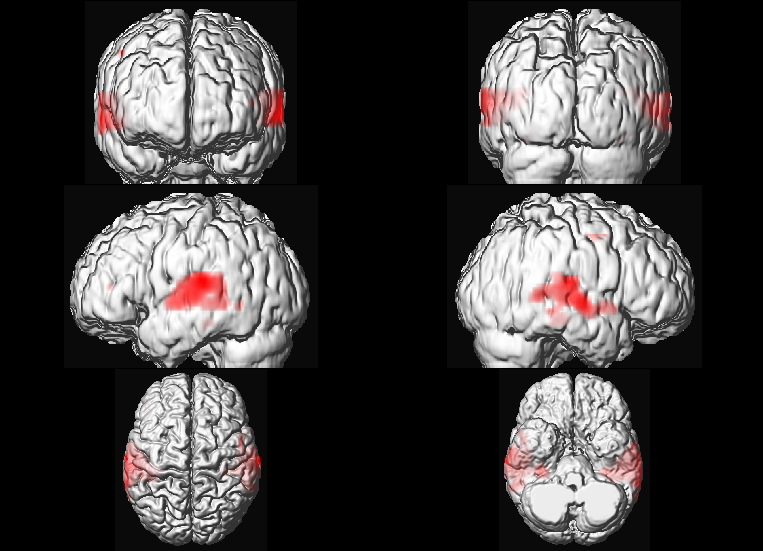
\includegraphics[width=100mm]{auditory/render}
\caption{\em Render. \label{aud_render} }
\end{center}
\end{figure}

\subsection{Miscellaneous}

Other options (in the results controls panel):

\bi
\item{clear: clears lower subpanel of Graphics window}
\item{exit: exits the results section}
\item{? : launches spm-results-ui help}
\ei

\section{Bayesian analysis}

\subsection{Specification}

Press the `Specify 1st-level' button. This will call up an fMRI specification job in the graphics window. Then

\bi
\item{Open the fMRI model specification option}
\item{Load the `specify.mat' job file created for the classical analysis}
\item{Open `Subject/Session', highlight `Scans'} \item{Deselect the smoothed functional images using the `unselect all' option available from a right mouse click in the SPM file selector (bottom window)}
\item{Select the unsmoothed functional images using the \verb!^w.*! filter and `select all' option available from a right mouse click in the SPM file selector (top right window)\footnote{Remember not to select the first 12 scans, scans 4 to 15, as these may contain T1 effects. This can be done during selection or by first moving the files to a different directory.}. The Bayesian analysis uses a spatial prior where the spatial regularity in the signal is estimated from the data. It is therefore not necessary to create smoothed images if you are only going to do a Bayesian analysis.}
\item{Press `Done'}
\item{Highlight `Directory' and select the \verb!DIR/bayesian! directory you created earlier (you will first need to deselect the \verb!DIR/classical! directory).}
\item{Save the job as \verb!specify_bayesian.mat! and press `Run'}
\ei

\subsection{Estimation}

Press the `Estimate' button. This will call up the specification of an fMRI estimation job in the graphics window. Then

\bi
\item{Open the `fMRI model estimation' option}
\item{Highlight the `Select SPM.mat' option and then choose the SPM.mat file saved in the \verb!DIR/bayesian! directory}
\item{Highlight `Method' and select the `Choose Bayesian 1st-level' option.}
\item{Open the newly created `Bayesian 1st-level' option, highlight `AR model order' and select 0. This data set has a TR=7s, so is unlikely to have temporally autocorrelated errors.}
\item{Save the job as \verb!estimate_bayesian.job! and press `Run'.}
\ei

SPM will write a number of files into the output directory including 

\bi
\item{An \verb!SPM.mat! file.}
\item{Images of estimated regression coefficients  \verb!Cbeta_0001.img! and \verb!Cbeta_0002.img!. These filenames are prefixed with a `C' indicating that these are the mean values of the `Conditional' or `Posterior' density.}
\item{Images of error bars/standard deviations on the regression coefficients \verb!SDbeta_0001.img! and \verb!SDbeta_0002.img!.}
\item{An image of the standard deviation of the error \verb!Sess1_SDerror.img!.}
\item{An image \verb!mask.img! indicating which voxels were included in the analysis.}
\ei

\subsection{Inference}

After estimation:

\bi
\item{Press `Results'}
\item{Select the \verb!SPM.mat! file created in the last section}
\item{Select `Define new contrast'}
\item{Enter the name `active $>$ rest'}
\item{Enter the value `1', press `Submit', `OK', `Done'}
\item{\em Mask with other contrast ? [Yes/No]}
\item{Specify No}
\item{Title for comparison, accept the default}
\item{\em Effect size threshold for PPM}
\item{Enter the value 2}
\item{\em Posterior probability threshold for PPM}
\item{Enter the value 0.99}
\item{\em Extent threshold [0]}
\item{Accept the default value}
\item{\em Plot effect size [Yes/No]}
\item{Select the default `Yes'}
\ei

SPM will then plot a map of effect sizes at voxels where it is 99\% sure that the effect size is greater than 2\% of the global mean. This is a large activation. Then use overlays, sections, select the normalised structural image created earlier and move the cursor to the activation in the left hemisphere. This should create the plot shown in Figure~\ref{aud_bayes}

\begin{figure}
\begin{center}
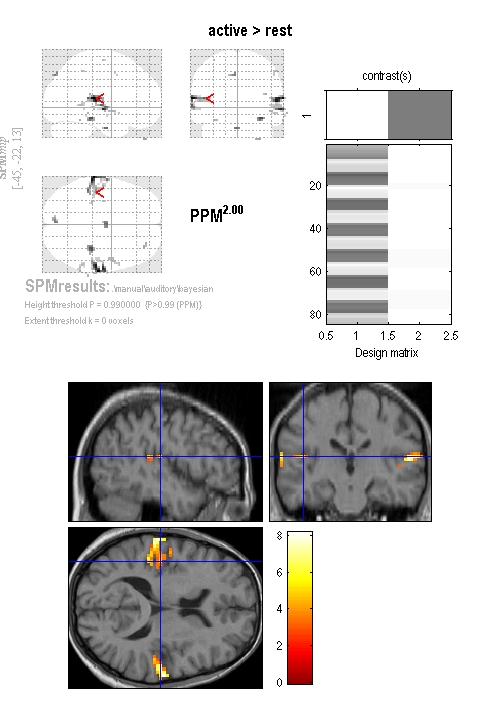
\includegraphics[width=100mm]{auditory/aud_bayes}
\caption{\em {\bf Bayesian analysis:} MIP and overlay of effect sizes at voxels where SPM is 99\% sure that the effect size is greater than 2\% of the global mean. \label{aud_bayes} }
\end{center}
\end{figure}

It is also possible to look for regions where responses in the active condition are different to those at rest. Active responses could be greater or smaller.

\bi
\item{Press `Results'}
\item{Select the \verb!SPM.mat! file created in the last section}
\item{Select `Define new contrast' and highlight the `F' radio button}
\item{Enter the name `active != rest'}
\item{Enter the value `1', press `Submit', `OK', `Done'}
\item{\em Mask with other contrast ? [Yes/No]}
\item{Specify No}
\item{Title for comparison, accept the default}
\item{\em Posterior probability threshold for PPM}
\item{Accept the default value\footnote{The default PPM threshold is set to $1-1/S$ where S is the number of voxels in the volume being analysed. The rationale for this is that inference is based on an approximate posterior distribution, $Q$, which factorises across voxels. The approximate posterior is chosen to best match the true posterior in the sense of KL-divergence. Given the factorisation in $Q$, the expected number of false positives in the PPM is 1. }}
\item{\em Extent threshold [0]}
\item{Accept the default value,0}
\item{\em Plot effect size [Yes/No]}
\item{Select the default `Yes'.}
\ei

SPM will then plot a map of $\chi^2$ statistic values at above threshold voxels. Then use overlays, sections, select the normalised structural image created earlier and move the cursor to the activation in the left hemisphere. This should create the plot shown in Figure~\ref{aud_bayes2}

\begin{figure}
\begin{center}
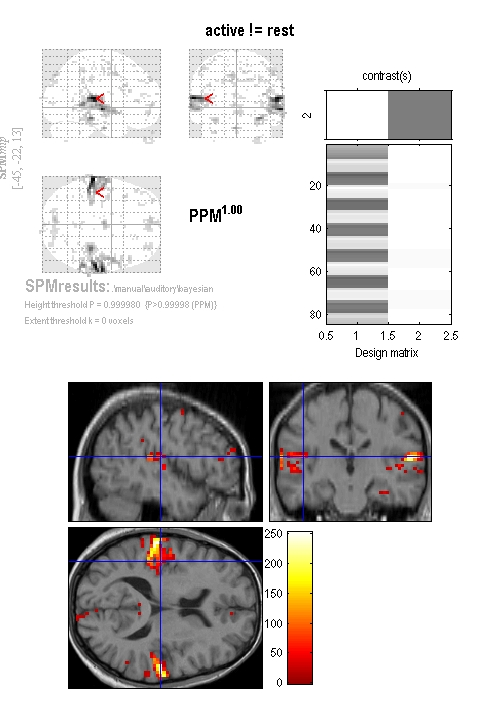
\includegraphics[width=100mm]{auditory/aud_bayes2}
\caption{\em {\bf Two-sided Bayesian analysis:} MIP and overlay of $\chi^2$ statistic values at above threshold voxels. This shows regions where activity is different between active and rest conditions, whether positive or negative. \label{aud_bayes2} }
\end{center}
\end{figure}

When you revisit the contrast manager this contrast will be referred to as a `P' contrast, rather than an `F' contrast. This indicates that Bayes rule is used to make the inference. To indicate that we are testing a two-sided effect it is advisable to make this clear when naming the contrast (as we have done with the label `active != rest).

